
\subsubsection{Organisation générale du jeu}

Concernant l'organisation générale du jeu, nous avons fait les choix suivants:
\begin{itemize}
	\item Je joueur à un point de départ fixe. En effet, celui-ci commence le jeu sur une île à partir de laquelle il pourra se diriger vers les autres îles.
	\item Celui-ci se retrouve dans une zone;
	\item A partir de là, une question est choisie aléatoirement parmi une liste de questions relative à cette zone et les propositions à cette question sont présentées au joueur.
	\item certaines des propositions peuvent ne s'afficher 
	\item Le joueur choisi une des propositions et en fonction de son choix, une des zones cible est choisie aléatoirement parmi la liste de zones relative à la proposition.
	\item Le joueur arrive à nouveau sur une zone ,et à nouveau une question est choisie aléatoirement.   
\end{itemize}
\begin{figure}[h]
	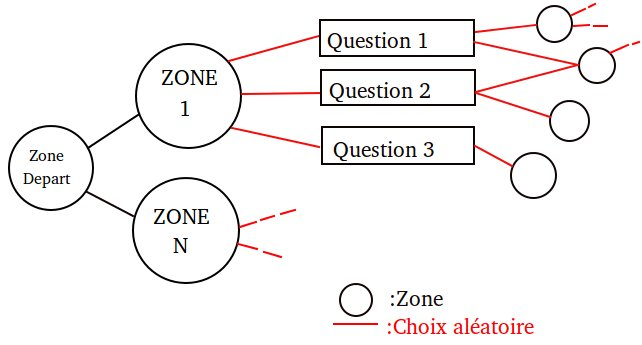
\includegraphics[scale=0.7]{figures/schema-organisation.jpg}
	\caption{Schéma de l'organisation du jeu }
\end{figure}